\documentclass[uplatex,10pt,a4paper,twocolumn]{jsarticle}
%
\usepackage{amsmath}
\usepackage{bm}
%
\def\diff{\mathrm d}
\def\dd#1#2{\dfrac{\diff #1}{\diff #2}}
\def\pp#1#2{\dfrac{\partial #1}{\partial #2}}
\def\dd2#1#2{\dfrac{\diff^2 #1}{\diff #2^2}}
\def\pp2#1#2{\dfrac{\partial^2 #1}{\partial #2^2}}
%
\usepackage[dvipdfmx]{graphicx, color}
%
\pagestyle{empty}
\usepackage[truedimen,margin=25truemm]{geometry}

\renewcommand{\baselinestretch}{0.9} % 全体の行間調整
\renewcommand{\figurename}{Fig.}
\renewcommand{\tablename}{Tab.}
\usepackage{setspace}

\graphicspath{{../../figures/}}

\begin{document}
\twocolumn[

\begin{center}
{\Large MD シミュレーションによるネットワークポリマーの緩和挙動}
\end{center}
\begin{flushright}
{\large 東亞合成  $\bigcirc$佐々木裕}
\end{flushright}

%\vspace{1mm}

\begin{center}
{\large Relaxation Characteristics of Network Polymers with random connectivity \\using Molecular Dynamics Simulations}

$\bigcirc$H. Sasaki\\
Toagosei Co., Ltd
\end{center}
\vspace{2mm}

]


\begin{spacing}{0.95}
ABSTRACT: 
Existence of mechanical hysteresis is believed to be one of a key to achieve high durability for rubber materials.
% For hysteresis cycle, added fillers are known to play an important roll in meso-scale region response against local stress.
% Our question is ``Is there any other mechanism to enhance durability in micro-scale region such as size of polymer chains?''.

``Phantom Network Model'', in which fluctuation of junction point is rather high, seems to be a good candidate for micro-scale energy dissipation.
Employing molecular dynamics simulation method, relaxation characteristics of ``Phantom Network Model'' was investigated.
\end{spacing}

\section{はじめに}
近年、ソフトマターの階層的な構造設計の考え方が深化し、力学特性に優れたネットワークポリマーの材料設計にも応用されている。
旧知の材料であるゴムの大きな破壊靭性の由来については、 ヒステリシスロスのようなエネルギー散逸により亀裂進展が抑制されるという Andrews モデルが提案されている\cite{andrews}。
また、ゴム系材料の破壊において時間温度換算則が大変形を伴う破壊挙動にも成立し、室温では容易に破断する SBR がガラス転移温度に近い低温での伸長では高い伸びと強度を示すことも報告されている~\cite{smith}。

ゴム弾性の古典的なモデルである ``Affine Network Model'' からの発展形として、結節点の揺らぎに注目した``Phantom Network Model: PNM''が提案され、Flory によればメルト状態と同一なストランドのゆらぎを有するランダムネットワークにおいて PNM のふるまいを示すとされている~\cite{flory}。
我々は、この結節点のゆらぎ由来の散逸が、分子鎖描像のようなミクロなスケールでの粘弾性的な挙動のモデルとなりうるのではないかと考え、これまで検討を進めている。

以前に、ネットワーク構造の接続性をランダムへと変えることで架橋欠損のないネットワークを作成して PNM を再現できることを報告した~\cite{sasaki}。
本報告では、ランダムな接続性を有するネットワークポリマーの力学特性と緩和挙動との関係について、MD シミュレーションにより検討した結果について報告する。

% ゴムの大きな破壊靭性の由来については、 ヒステリシスロスのようなエネルギー散逸により亀裂進展が抑制されるという Andrews モデルが提案されている~\cite{Andrews1977}。
% ゴムへのフィラーの添加がヒステリシスの主要な発生原因とされ~\cite{Grosch1968}、その発現機構の 1 つとしてフィラー近傍でのナノキャビティーの開閉も報告されている~\cite{Zhang2013}。
% フィラー由来の靭性向上効果はメゾスケール領域の挙動であると考えられているが、このようなエネルギー散逸挙動はメゾスケールでしか発現しないのであろうか?

% ゴム弾性の古典的なモデルは、ガウス鎖をストランドとしたネットワークの結節点のミクロな変形がマクロな変形と相似でアフィン変形するとした``Affine Network Model: ANM'' である。%~\cite{Flory1953}。
% この古典モデルからの発展形として、結節点の揺らぎに注目しミクロな変形がマクロと異なるとした``Phantom Network Model: PNM''が提案されている~\cite{James1943}。
% Flory によれば、メルト状態と同一なストランドのゆらぎを有するランダムネットワークにおいて PNM のふるまいを示すとされている~\cite{Flory1976}。

% 我々は、この結節点のゆらぎ由来の散逸が、分子鎖描像のようなミクロなスケールでの粘弾性的なエネルギー散逸モデルとなりうるのではないかと考え、これまで検討を進めている。
% 以前に、規則構造ネットワークをベースとしてユニットセル間における規則性をランダムへと変えることで架橋欠損のないネットワークを作成して PNM を再現できることを報告した。

% 本報告では、ランダムな接続性を有するネットワークポリマーの緩和挙動について、MD シミュレーションにより検討した結果について報告する。

\section{シミュレーション}

% ランダムな結合性を有するネットワークを作成し、その平衡状態および一軸伸2長時の振る舞いについて、OCTA 上の COGNAC シミュレーターを用いた分子動力学シミュレーションにより評価した。

既報~\cite{sasaki}に従い、ランダムな接続性を有する 4 分岐のネットワークを作成し、その平衡状態および変形(一軸伸張およびずりせん断)時の振る舞いについて、OCTA 上の COGNAC シミュレーターを用いた分子動力学シミュレーションにより評価した。

\subsection{ネットワークモデルの作成}

% 任意の分岐数$f$($f=3\sim6$)の結節点からなる規則構造を有するネットワークより、
以下のアルゴリズムでランダムな結合性を導入した。

% \vspace{-2mm}
\begin{enumerate}
\item
実空間での初期構造を体心立方構造の各格子点をストランドでつないだ「八本鎖モデル」として、それに対応するように任意の分岐数のトポロジーモデルを作成。
% (Fig. \ref{fig:topo})。
\item
代数的連結性を指標として連結性を維持しながらストランド交換し、結節点の結合性にランダム性を導入。
% (Fig. \ref{fig:exc})。
\item
トポロジーモデルに対応して実空間の構造作成。
\end{enumerate}

% \vspace{-8mm}
% \begin{figure}[htb]
% 	\begin{center}
% 	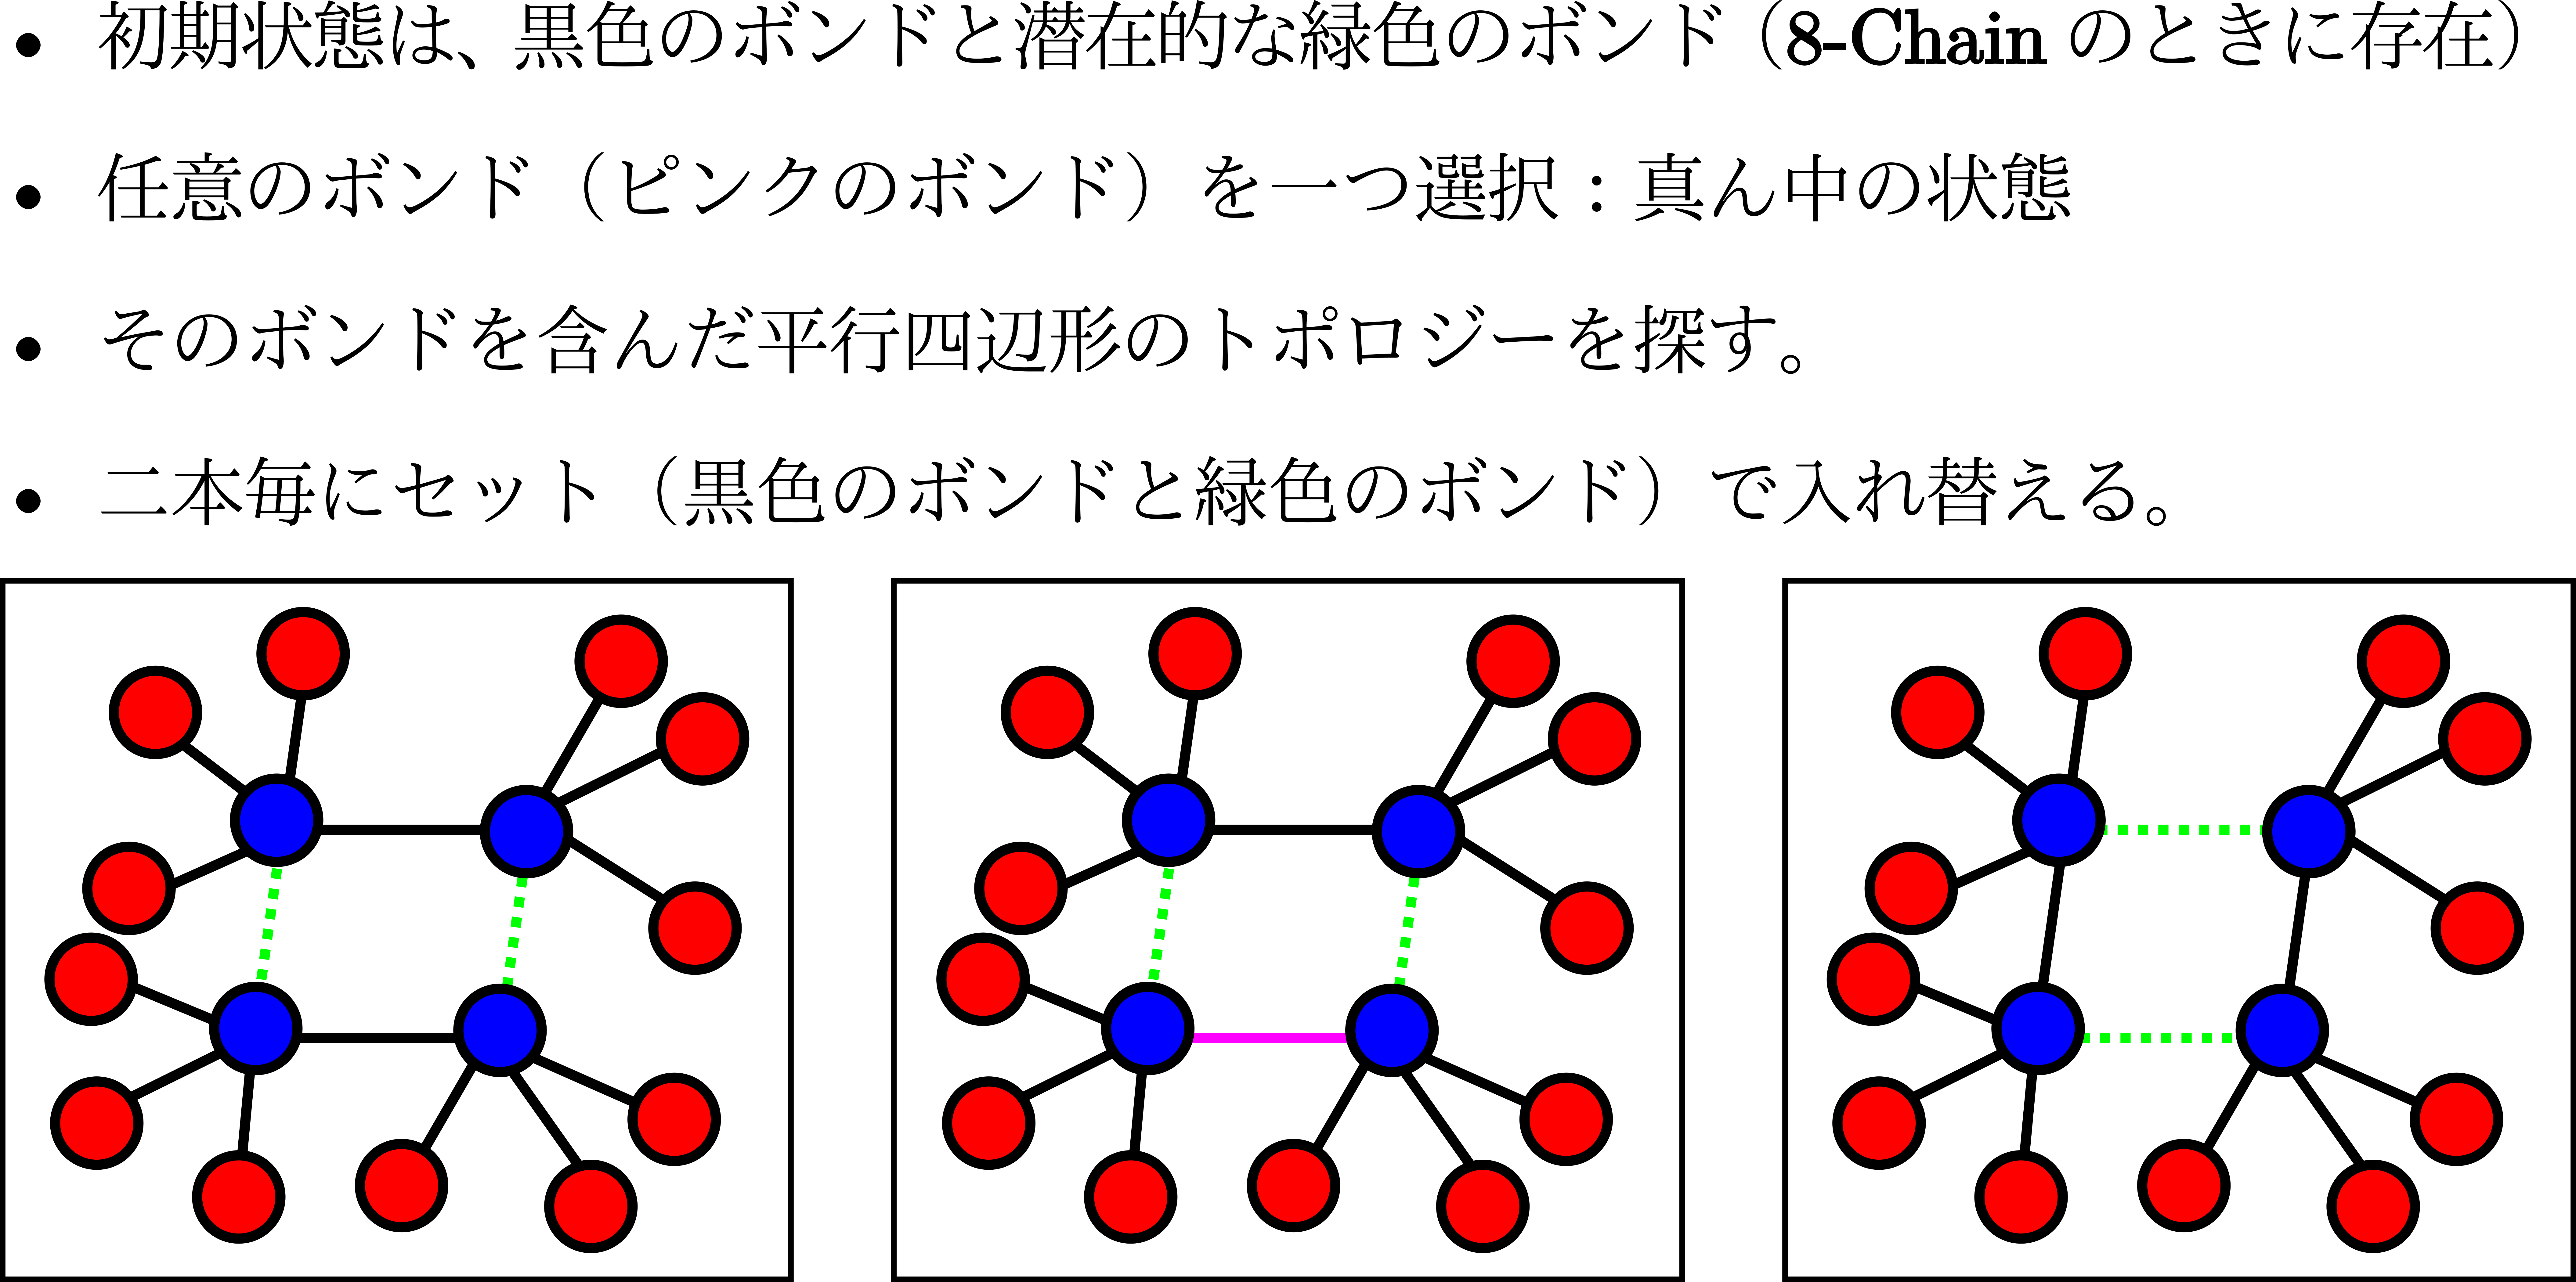
\includegraphics[width=.42\textwidth]{bond_exchg.png}
% 	\caption{Strand Exchange Procedure}
% 	\label{fig:exc}
% 	\end{center}
% \end{figure}
% \vspace{-5mm}

\subsection{初期構造の作成}
セグメント数 N=20 のストランドを用いネットワークの多重度を 3 とすることで、KG 鎖の一般的な密度 ($\rho$=0.85) の四分岐モデルを作成した。

\subsection{ポテンシャルの設定}
セグメント間の非結合ポテンシャルに斥力($r_c = 2^{1/6}\sigma$)である LJ ポテンシャル $U_{LJ}(r_{ij})$、ボンドポテンシャルには FENE-LJ ポテンシャルを用いて KG 鎖とした。
なお、初期構造の緩和は Auhl 等の方法~\cite{Auhl} に従い force-capped-LJ ポテンシャルを用いて、段階的にす抜け鎖から絡み合い鎖へと遷移させた。
Kr\"{o}ger らの方法~\cite{Kroger} によりストランド同士の絡み合いを評価して、対応するホモポリマーメルトと同程度であることを確認した。


\section{結果と考察}

\subsection{力学応答の評価}
4 分岐のネットワークポリマーの変形速度の異なるせん断変形($\dot{\gamma} = 1e^{-2} \sim 5^{e-5}$)時の SS カーブを、各種モデルの理論曲線と共に Fig. \ref{fig:deform} に示した。
\newpage

\begin{figure}[htb]
	\begin{center}
	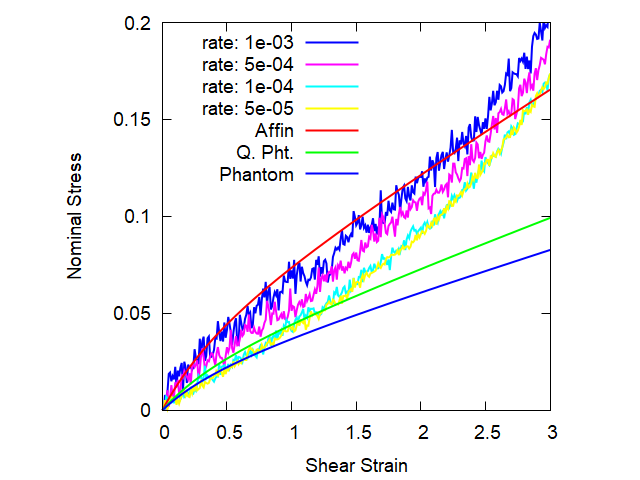
\includegraphics[width=.42\textwidth]{Shear_Random_4chain_N20.png}
	\caption{Stress-Strain Curves for 4-chain NW at varied shear rate ($\dot{\gamma}: 1e^{-2} \sim 5^{e-5}$)}
	\label{fig:deform}
	\end{center}
\end{figure}
\vspace{-5mm}

変形速度の低減により、$\gamma<1$ 程度の小さなひずみでは PNM に漸近していた。


\vspace{-2mm}
\begin{figure}[htb]
	\begin{center}
	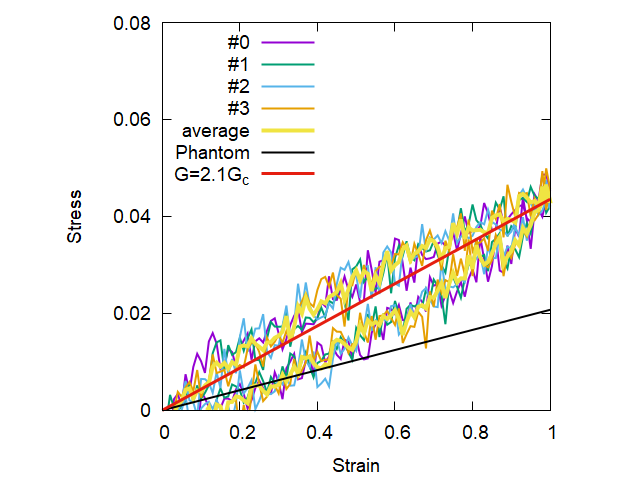
\includegraphics[width=.42\textwidth]{CyclicDeform_4chain_rate_2e-4.png}
	\caption{Hysteresis Curves for 4-chain NW by Cyclic Shear ($\gamma = 1$) = shear rate $\dot{\gamma} = 2e^{-4}$}
	\label{fig:hyst}
	\end{center}
\end{figure}
\vspace{-5mm}

PNM へと漸近する変形速度 ($\dot{\gamma} = 2e^{-4}$) で周期的な変形 ($\gamma = 1$) を付与した結果を示した (Fig. \ref{fig:hyst})。

複数回の変形に対しても迅速な回復を伴った力学的ヒステリシス (Hysteresis loss $\simeq$ 0.34) を示すことが確認できた。

\vspace{-2mm}
\begin{figure}[htb]
\centering
	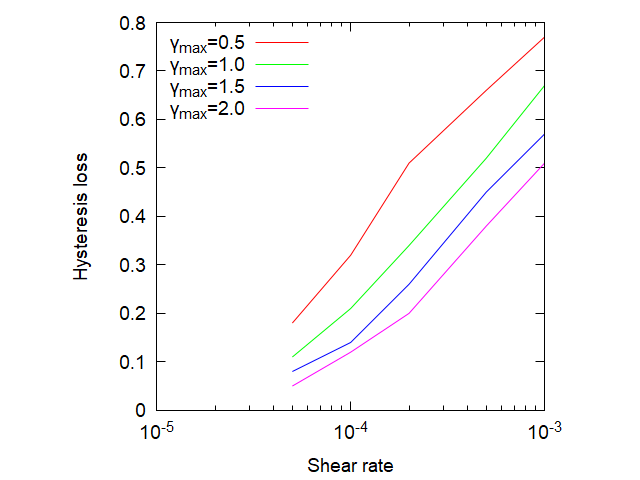
\includegraphics[width=.42\textwidth]{hyst_shear.png}
\caption{Hysteresis losses for varied shear rates and maximum strains}
\label{fig:hystloss}
\end{figure}
\vspace{-5mm}

各種の変形条件での力学的ヒステリシスの振る舞いを、Fig. \ref{fig:hystloss} に示した。

変形速度の低下に伴いヒステリシスロスは減少し、$\dot{\gamma} \sim 1e^{-5}$ 程度の時間スケールで消失するようであった。

\subsection{最長緩和時間の検討}

長時間緩和後の平衡構造において、ラウスモード(p=1)の自己相関関数から最長緩和時間 ($\tau$) について評価した結果を Fig. \ref{fig:ac-xp} に示した。
なお、ネットワークのストランドは空間的に拘束されておりその相関は長時間極限で一定値に収束するため、それを差し引いて緩和成分の評価を行い、$\tau \simeq 6.5e^{4}$ を得た。
\vspace{-1mm}
\begin{figure}[htb]
\centering
	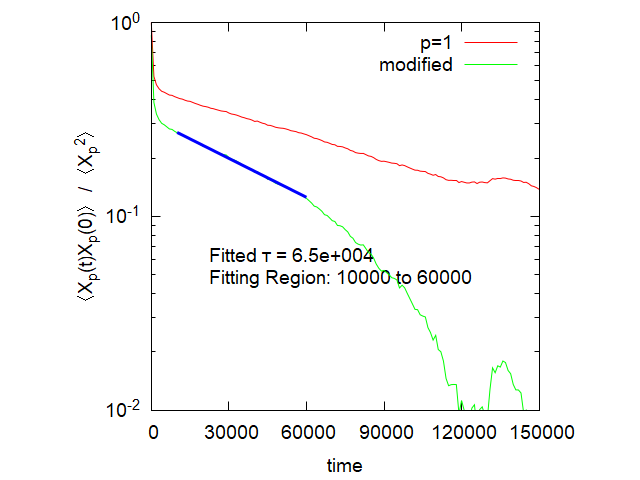
\includegraphics[width=.42\textwidth]{Xp_1_org.png}
\caption{Auto Correlation of Rouse mode (p=1) for equilibrated structure}
\label{fig:ac-xp}
\end{figure}
\vspace{-5mm}

この緩和時間の長時間化はネットワーク構造に起因した架橋点の運動性の低下によるものと想定でき、長鎖のホモポリマーメルトでの絡み合いに起因したラウスモードのふるまい~\cite{rubinstein} と合致していた。
また、この値の逆数は前述のヒステリシスロスが消失する変形速度と対応するものと考えられた。


また、高次のラウスモードの緩和について検討した結果についても、報告する予定である。

\begin{thebibliography}{99}
	\bibitem{andrews} E. H. Andrews, Y. Fukahori, Journal of Materials Science, 12, 1307 (1977)
	\bibitem{smith} T. L. Smith, R. A. Dickie, Journal of Polymer Science Part A-2: Polymer Physics, 7, 635 (1969)
	\bibitem{flory} P. J. Flory, Proceedings of the Royal Society of London. Series A, 351, 351 (1976)
	\bibitem{sasaki} 佐々木裕, 第69回レオロジー討論会 要旨集 (2021)
	\bibitem{Auhl} R. Auhl et al., Journal of Chemical Physics, 119, 12718 (2003)
	\bibitem{Kroger} S. Shanbhag, M. Kr\"{o}ger, Macromolecules 40 2897 (2007)
	\bibitem{rubinstein} J. T. Kalathi et al., Macromolecules 47 6925 (2014)
\end{thebibliography}
% \bibliographystyle{../achemso}
% \bibliography{C:/texlive/texmf-local/bibtex/bib/library.bib}
\end{document}